%%%%%%%%%%%%%%%%% Préambule %%%%%%%%%%%%%%%%%%%%%%%%%%%%%
\documentclass[12pt,a4paper]{report}
\usepackage[hmargin=2cm,vmargin=2cm]{geometry}  
%%%%%%%%%%% marges horizontales et verticales
\usepackage{subfigure}
\usepackage{tabto}
\usepackage{amsmath,amsthm}
\usepackage{amsfonts}
\usepackage{amssymb,amsmath,latexsym}
\usepackage{graphics}							
\usepackage[pdftex]{graphicx}					
\usepackage[T1]{fontenc}
\usepackage{ae,aecompl}
\usepackage[francais]{babel}
\usepackage[linesnumbered,ruled]{algorithm2e}	
\bibliographystyle{style utilis\'e}
\numberwithin{equation}{subsection}
\newtheorem{thm}{Th\'{e}or\`{e}me}[section]
\newtheorem{cor}[thm]{Corollaire}
\newtheorem{lem}[thm]{Lemme}
\newtheorem{prop}[thm]{Proposition}
\newtheorem{prob}{Probl\`{e}me}
\newtheorem{defn}[thm]{D\'{e}finition}
\newtheorem{rem}[thm]{Remarque}
\newtheorem{ex}{Exemple}
\numberwithin{equation}{section}
\newtheorem{nt}{Notation}
\usepackage[utf8]{inputenc}
\usepackage{setspace}
\onehalfspacing
\usepackage[T1]{fontenc}
\usepackage{hyperref}
\usepackage{fancyhdr}
\usepackage[utf8x]{inputenc}
\usepackage[T1]{fontenc}
\usepackage[francais]{babel}
\usepackage{graphicx}




\begin{document}



\begin{titlepage}
\begin{center}

\vfill

\includegraphics[width=0.75\textwidth]{fsa.png}

\large{\textbf{UniversitŽ Ibn Zohr\\
FacultŽ des Sciences Agadir\\
DŽpartement d'Informatiques\\
Filire Sciences MathŽmatiques et Informatique
}}

\vfill

\Large\textbf{Réduction de bruit de la vidéo\vspace{0.2in} par  filtre non local }

\vfill

\large{ Projet tutorŽ pr\'{e}par\'{e} par }

\textbf{Chaima Elmejgari et Nouhaila Hasssni }

\vspace{1.5cm}

\underline{ Sous la direction de }

\underline{Prof: M. El Oufdi Ahmed Fouad }

\vfill


Soutenu le : ... Mai 2020
\end{center}

\vfill

\noindent Devant le jury :


\bigskip

\begin{tabular}{ll}
Prof. ................................& Professeur ˆ la FacultŽ des sciences Agadir\\
Prof. .............& Professeur ˆ la   FacultŽ des sciences Agadir
\end{tabular}

\vfill
\begin{center}
\emph{AnnŽe Universitaire : 2019-2020}
\end{center}


\end{titlepage}



\vfill

\chapter*{Introduction}


\chapter*{Remerciements}

\tableofcontents
\chapter{Généralisation}
\section{Introduction}
Les images numériques sont présentées sous forme de matrices, cependant les
opérations, en particulier arithmétique, se font entre pixels, des deux images, situés aux
mêmes positions.
De ce fait, nous allons réserver ce chapitre à la présentation des notions générales liées
à l’image.

\section{Définition d’une image}

Une image numérique est un signal numérique composé d’unités élémentaires (appelées pixels) qui représentent chacun une portion de l’image. Contrairement au cas unidimensionnel, nous étudierons uniquement les images numériques (discrétes). \newline Une image numérique est définie par : \newline– le nombre de pixels qui la composent en largeur et en hauteur, \newline– l’étendue des teintes de gris ou des couleurs que peut prendre chaque pixel (on parle de dynamique de l’image).
\newline
\begin{figure}[!h]
    \centering
    \begin{center}
        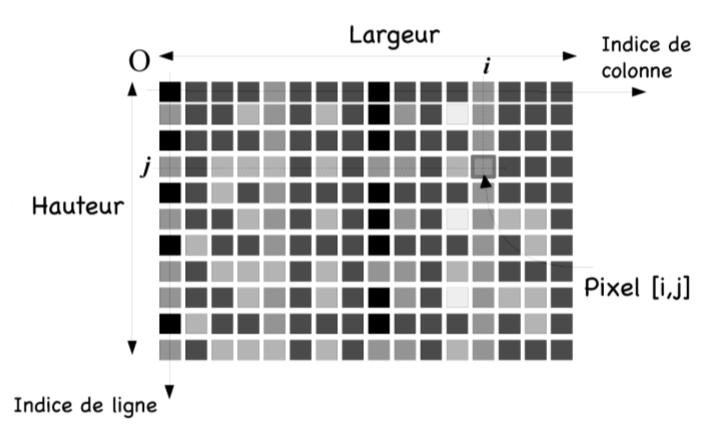
\includegraphics[height=5cm,width=10cm\textwidth]{imagenum.png}
    \end{center}
    \caption{Capteurs}
\end{figure}


\subsection{Les images binaires (noir ou blanc)}
\begin{figure}[!h]
    \centering
    \begin{minipage}[b]{0.3\textwidth}
        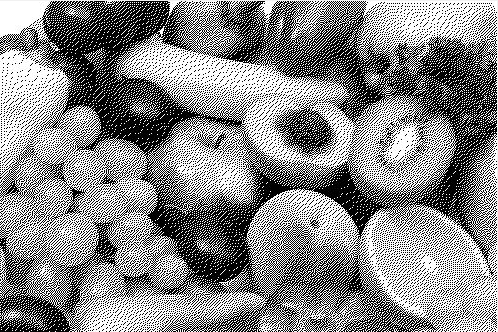
\includegraphics[height=3.25cm,width=3.5cm\textwidth]{noir1.png}
    \end{minipage}
    \begin{minipage}[b]{0.3\textwidth}
        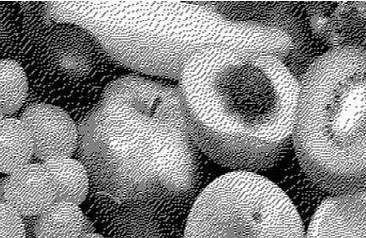
\includegraphics[height=3.25cm,width=3.5cm\textwidth]{noir3.png}
    \end{minipage}
    \begin{minipage}[b]{0.3\textwidth}
        
\includegraphics[height=3.25cm,width=3.5cm\textwidth]{noir2.png}
    \end{minipage}
    \caption{Les images binaires (noir ou blanc) }
\end{figure}

Est une image en noir et blanc, dans lequel chaque pixel est soit noir, soit blanc.
\subsection{Les images en niveaux de gris}
\begin{figure}[!h]
    \centering
    \begin{minipage}[b]{0.3\textwidth}
        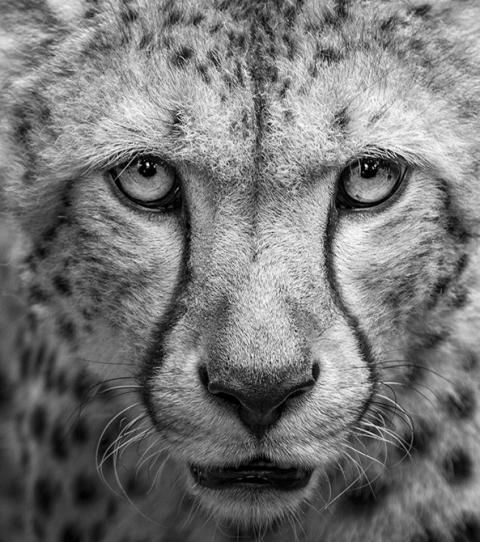
\includegraphics[height=3.25cm,width=3.5cm \textwidth]{gris.png}
    \end{minipage}
    \begin{minipage}[b]{0.3\textwidth}
        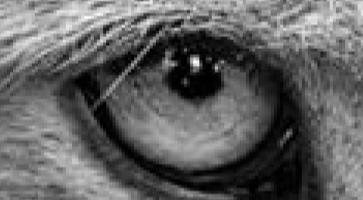
\includegraphics[height=3.25cm ,width=3.5cm \textwidth]{gray3.png}
    \end{minipage}
    \begin{minipage}[b]{0.3\textwidth}
        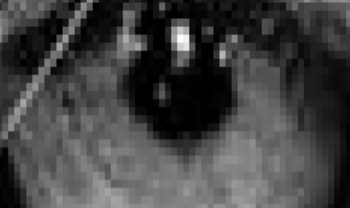
\includegraphics[height=3.25cm, width=3.5cm \textwidth]{gray2.png}
    \end{minipage}
    \caption{Les images en niveaux de gris}
\end{figure}
\raggedrightLes images en niveaux de gris renferment 256 teintes de gris. Par convention la valeur zéro représente le noir et la valeur 255 le blanc. En effet chaque entier représentant un niveau de gris est codé sur 8 bits. 
\newline Il est donc compris entre 0 et 2^{8}-1=255. On peut coder une image en niveaux de gris sur 16 bits (0 ≤ n ≤ 216 - 1) ou sur 2 bits, dans ce dernier cas le niveau de gris vaut 0 ou 1 : il s'agit alors d'une image binaire (Noir et Blanc).
 
\subsection{Les images couleurs}
\begin{figure}[!h]
    \centering
    \begin{minipage}[b]{0.3\textwidth}
        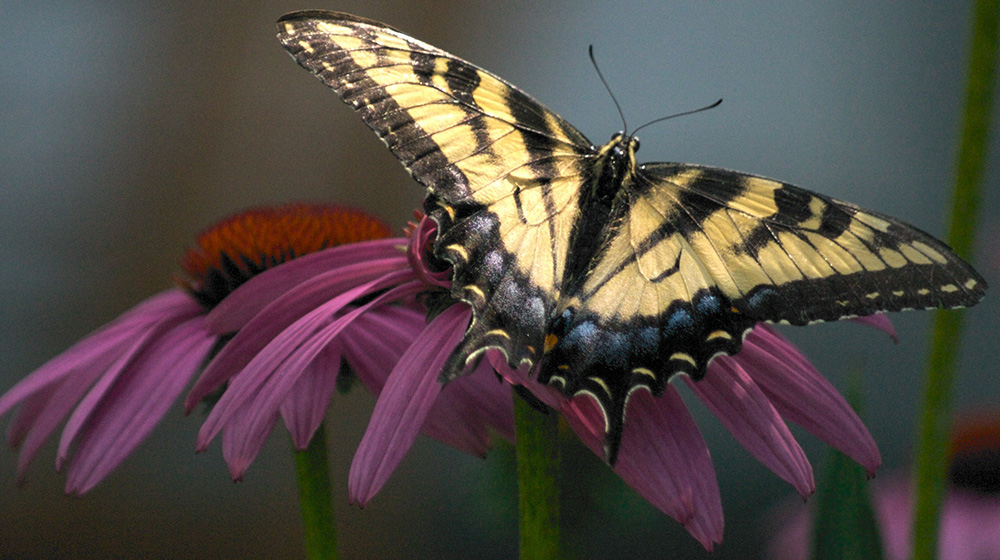
\includegraphics[height=3.25cm,width=3.5cm\textwidth]{couleur1.jpg}
    \end{minipage}
    \begin{minipage}[b]{0.3\textwidth}
        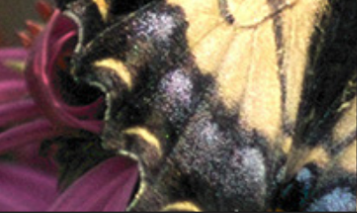
\includegraphics[height=3.25cm,width=3.5cm\textwidth]{couleur2.png}
    \end{minipage}
    \begin{minipage}[b]{0.3\textwidth}
        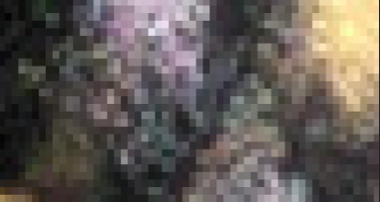
\includegraphics[height=3.25cm,width=3.5cm\textwidth]{couleur3.png}
    \end{minipage}
    \caption{Les images couleurs}
\end{figure}
Pour chaque pixel, on code en binaire chacune des 3 valeurs des composantes R, V, B (Rouge, Vert, Blue) de la couleur du pixel. Le code binaire de l'image est obtenu en indiquant successivement pour chaque pixel le code binaire des 3 composantes. Si on code chaque composante sur 8 bits, chaque pixel sera donc représenté par 24 bits.

\newpage
\newline
\newline
\newline

\section{Formats d’images}
Un format d'image est une représentation informatique de l'image, associée à des
informations sur la façon dont l'image est codée et fournissant éventuellement des indications sur la
manière de la décoder et de la manipuler.
\\ 
Il existe un grand nombre de formats. Voici les plus utilisés :\\

\begin{tabular}{|p{1.5cm}|p{4cm}|p{2cm}|p{2cm}|p{4cm}|}
\hline
format & Compression des
données & Nb de
couleurs & Affichage
progressif & Usage \\
\hline
BMP & Non compressé & de 2 à 16
millions & non & Image non dégradée mais très lourde.Stokage \\
\hline
JPEG & Réglable,avec perte de qualité.Plus la compression est importante,plus l'image est dégradée. & 16millions & oui & Tous usages,selon compression.Images"naturelles".\\
\hline
GIF & Oui,sans perte de qualité & de 2 à 256 avec palette & oui & Logos et Internet.Supporte les animations et la transparence \\
\hline
TIFF & Réglable, au choix sans perte ou avec perte de qualité & 16 millions & non & Tous sauf Internet \\
\hline
PNG & Oui, sans perte de qualité & de 2 à 256 ou 16 millions & oui & Tous, recommandé Internet mais incompatible avec les navigateurs anciens. Supporte la transparence. \\
\hline
\end{tabular}
\newline
\newline



\newpage
\section{ Traitement et acquisition d'image}
 Il existe trois agencements de capteurs principaux utilisés pour transformer l'énergie d'éclairage en images numériques.  \newline- Capteur d'imagerie unique. \newline- Capteur de ligne. \newline- Capteur matriciel.
\begin{figure}[!h]
    \centering
    \begin{center}
        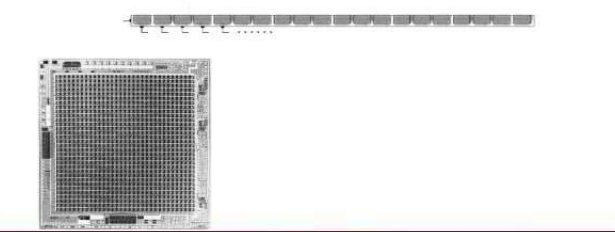
\includegraphics[height=5cm,width=10cm\textwidth]{capteur1.png}
    \end{center}
    \caption{Capteurs}
\end{figure}
\subsection{Processus d'acquisition d'images}
L'énergie entrante est transformée en tension par la combinaison de l'énergie électrique d'entrée et d'un matériau de capteur sensible au type particulier d'énergie détecté.  \newline
La forme d'onde de la tension de sortie est la réponse du ou des capteurs, et une quantité numérique est obtenue à partir de chaque capteur en numérisant sa réponse.
\newline
\newline
\subsection{Acquisition d'image Utilisation d'un seul capteur }
 Le plus familier Capteur de ce type est la photodiode, qui est construite en matériaux de silicium et dont la forme d'onde de tension de sortie est proportionnelle à la lumière. L'utilisation d'un filtre devant un capteur améliore la sélectivité. Afin de générer une image 2D à l'aide d'un seul capteur, il doit y avoir des déplacements relatifs dans les directions X et Y entre le capteur et la zone à imager.
 \begin{figure}[!h]
    \centering
    \begin{center}
        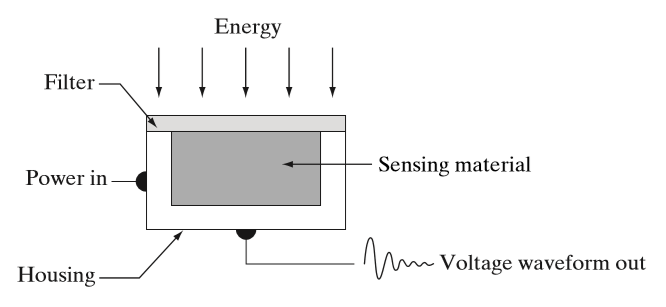
\includegraphics[height=5cm,width=10cm\textwidth]{capteur2.png}
    \end{center}
    \caption{Capteur d'imagerie unique}
\end{figure}
 \newline
\newline
\newline
\newline
\newline

\subsection{Acquisition d'image Utilisation  Capteur matriciel}
L'acquisition d'image est la création d'une représentation codée numériquement des caractéristiques visuelles d'un objet,
 comme une scène physique ou la structure intérieure d'un objet.

\begin{figure}[h!]
    \centering
    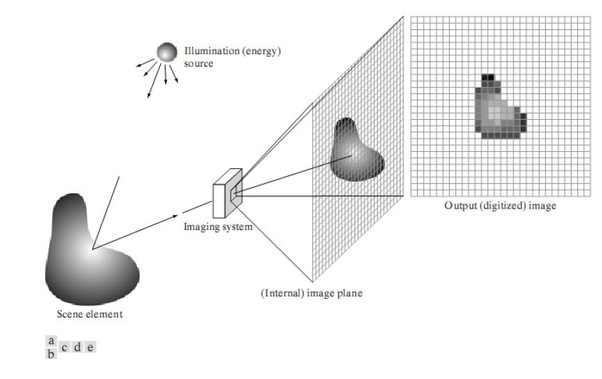
\includegraphics[width=.9\textwidth]{m.jpg}
   
     \caption{le processus d'acquisition d'images numériques}
\end{figure}
\newline
chaque appareil photo numérique possède un capteur qui convertit la lumière en charges électriques.Une façon simplifiée de penser à ces capteurs est de penser à un tableau 2D de milliers ou des millions de minuscules cellules solaires.
\newline

Il existe deux grandes familles des capteurs CCD et CMOS:\newline
Les capteurs CCD créent des images de haute qualité et à faible bruit.\newline
CMOS les capteurs sont généralement plus sensibles au bruit.
\newline

Un CCD transporte la charge à travers la puce etle lit dans un coin du tableau.Un analogique-numérique convertisseur (ADC) transforme 
ensuite la valeur de chaque pixel en un valeur numérique en mesurant le montant de la charge àchaque photosite et convertir cette mesure enforme binaire.\newline
Les appareils CMOS utilisent plusieurs transistors à chaque pixel pouramplifier et déplacer la charge en utilisant plus traditionnelfils.



\newpage
\section{Modèles de bruits de l’image}
\subsection{Le bruit additif}
Le bruit additif peut être défini de la façon suivante : étant données une image non bruitée R et I la même image avec bruit additif A.\newline
Alors chaque pixel j est caractérise par la relation : 

\begin{center}
    {\bfseries Ij=Aj+Rj}
\end{center}
\newline
\newline
 Ou Aj est une variable aléatoire de moyenne à 0.

\subsection{Le bruit multiplicatif}
Le bruit multiplicatif se défini de façon analogue : étant données une image non bruitée R et I la même image avec bruit multiplicatif Alors chaque pixel j est caractérise par la relation :\begin{center}
    {\bfseries Ij=Rj*Bj}
\end{center}
\newline
\newline Ou Bj est une variable aléatoire de moyenne égale à 1. La principale caractéristique de ce bruit est que les pixels d’une zone homogène seront d’autant plus bruités que leur niveau de gris est élevé.
\newpage
\section{Types de bruit}
La qualité de l’image numérique peut être dégradée par plusieurs types de bruits
survenus lors de l’acquisition et de la transmission. Ainsi il est important de connaître la
nature du bruit qui contamine l’image.
\newline
\subsection{Bruit Gaussien}
C’est le type de dégradation produite par les composantes électroniques du capteur
(relation linéaire avec la température du capteur) et liée à la limite en faible lumière de
celui-ci. C’est donc le bruit qui entache majoritairement les images numériques et que
nous considérerons plus tard.\newline
Pour créer synthétiquement ce bruit additif gaussien non corrélé (blanc), une variable
aléatoire gaussiene a été ajoutée par le système à l’image "idéale". Dans le cas précédent
des photos numériques, la source est la précision du capteur CCD ou CMOS mise en évidence par un gain élevé .
\begin{figure}[h!]
    \centering
    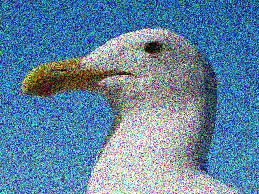
\includegraphics[width=.3\textwidth]{bruit_gaussien.jpg}
     \caption{bruit gaussien}
\end{figure}
\newline
\subsection{Bruit périodique}
Le bruit périodique dans une image est un bruit généré par un composant électronique , une machine ou un processus cyclique, la périodicité du bruit se constate par un motif de bruit se superposant sur des régions de l’image avec une fréquence spatiale déterminée.\\
\begin{figure}[h!]
    \centering
    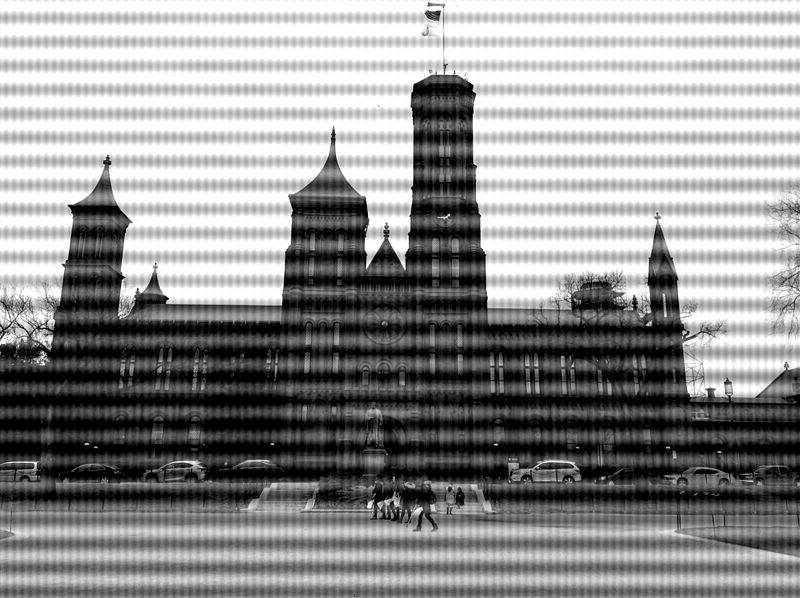
\includegraphics[width=.3\textwidth]{periodique.jpg}
     \caption{bruit périodique}
\end{figure}
\subsection{Bruit de chrominance}
C’est la composante colorée des pixels bruités : il est visible sous la forme de taches de
couleurs aléatoires.\\
\begin{figure}[h!]
    \centering
    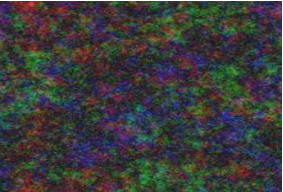
\includegraphics[width=.3\textwidth]{ch.PNG}
     \caption{bruit de chrominance}
\end{figure}
\newline
\subsection{Bruit de luminance}
C’est la composante lumineuse des pixels bruités : il est visible sous la forme de taches
plus foncées ou plus claires donnant un aspect granuleux à l'image.
\begin{figure}[h!]
    \centering
    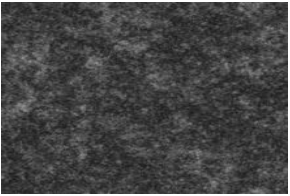
\includegraphics[width=.3\textwidth]{lu.PNG}
     \caption{bruit de luminance}
\end{figure}
\subsection{Bruit Poivre et sel}
Le bruit poivre et sel également appelé bruit impulsionnel, est une dégradation de l'image sous la forme de pixels noirs et blancs (d’où le nom poivre et sel) répartis d'une manière aléatoire dans l'image. Ce bruit est dû soit à des erreurs de transmission de données, soit aux dysfonctionnement ou à la présence de particules fines sur les éléments du capteur de la camera ou a des emplacements mémoire défectueux dans le matériel.
\begin{figure}[h!]
    \centering
    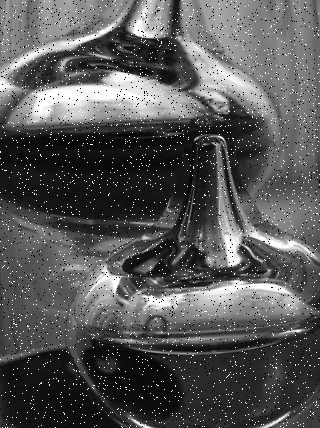
\includegraphics[height=3.25cm , width=.3\textwidth]{poi.png}
     \caption{bruit Poivre et sel}
\end{figure}
\newpage

\section{Conclusion}
Le bruit est une information indésirée qui pose un risque de perdre du contenu de l’image.\newline
Dans ce chapitre nous avons présenté les différents types de bruits, avec leurs
sources. \newline
Dans le chapitre suivant nous présentons les méthodes utilisées pour supprimer le bruit d’image avec une préservation des données utiles.
\chapter{Filtrage des images}
\section{Introduction}
Le filtrage est une approche qui consiste à éliminer la présence d’information parasite qui
s’ajoute de façon aléatoire à l’image, ce qui conduit à améliorer sa qualité. Comme nous pouvons
dire, le filtrage est une opération fondamentale en traitement d’image, il permet d’améliorer la
perception de certains détails, de réduire le bruit, de compenser certains défauts du capteur, etc… \newline
Dans ce chapitre nous nous intéressons avant tout aux généralités sur les catégories de
filtrage, puis nous étudions les filtres utilisés dans notre travail.
\newline

\section{ les Filtres locaux }
Dans cette partie, nous nous intéressons à des techniques qui font intervenir les
voisins d'un pixel, en plus du pixel considéré, pour modifier la valeur de ce pixel et fournir
une image améliorée.
On distingue dans ce type de filtre entre deux grandes catégories : les Filtres local
linéaires et Filtres local non-linéaires.
\newline

\subsection{filtre local linéaire }
\subsubsection{ \underline {filtre moyenneur}}
Appelé également mean filtering , averaging ou box filtering .
Ce filtrage remplace un pixel par la moyenne de lui meme et de ses voisins.
\newline
 Le filtre moyenneur permettant d'éliminer les hautes fréquences ,correspondant au bruit .son inconvénient est qu'il élimine également les hautes fréquences correspondants aux détailss de l'image : il rend ainsi l'image moins bruitée mais plus floue. 
\newline
Exemple:
\begin{figure}[h!]
    \centering
    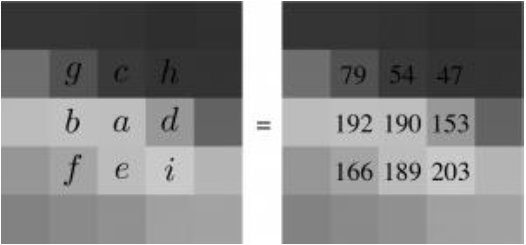
\includegraphics[width=.4\textwidth]{c.PNG}
   
    \label{fig3}
   \caption{EXEMPLE D’UN VOISINAGE 9 PIXELS}
\end{figure}
\newline

Dans notre exemple , cette moyenne vaut :

\newline 

\begin{center}
    (190+192+79+54+47+153+203+189+166)/9=141.4
\end{center}
\subsubsection{ \underline{ Filtre gaussien}}
Appelé également gaussian filtering .
le principe de ce filtrage est une convolution avec une gaussien. \newline
Nous rappelons l'expression d'une gaussienne s'écrit sous forme:
\begin{figure}[h!]
   $$G_{h}(\mathbf{x})=\frac{1}{\left(4 \pi h^{2}\right)} e^{-\frac{|x|^{2}}{4 h^{2}}}$$
\end{figure}
\newline
le lissage gaussien permet de corriger le bruit dans les parties homogénes des images mais est moins efficace que le lissage moyenneur .

\subsection{filtre local non linéaire}
\subsubsection{\underline{le filtrage anisotrope}}
est une méthode pour améliorer la qualité d'image des textures sur des surfaces d'infographie qui sont à des angles de vue obliques par rapport à la caméra où la projection de la texture (pas le polygone ou autre primitive) sur laquelle il est rendu) semble non orthogonal (d'où l'origine du mot: "un" pour non , "iso" pour pareil , et "tropique" du tropisme , relatif à la direction; le filtrage anisotrope ne filtre pas le même dans tous les sens).
\subsubsection{\underline{ le filtre médian}}
Ce filtre vise à remplacer la valeur du pixel central par la valeur médiane de la répartition (on trie les luminances dans l'ordre croissant) des niveaux de gris des pixels situés à l'intérieur de cette fenêtre, comme l’illustre la figure
suivante:\newline
\begin{figure}[!h]
    \centering
    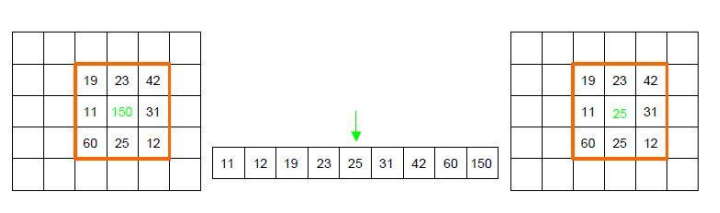
\includegraphics[height=4cm , width=.5\textwidth]{median1.png}
    \caption{FILTRE MEDIANLes}
\end{figure}
\newline
\newline
\newline
\newline
\newline
\newline
\newline
\newline
 pixels voisins sont triés suivant un ordre croissant de 11 vers 150, puis la valeur médiane
de la série numérique obtenue (25) devra remplacer la valeur 150.

\underline {Algorithme:}\newline1. trier les valeurs du voisinage par ordre croissant.\newline
2. sélectionner la médiane des valeurs
(La médiane est la valeur "milieu" : 50 % des valeurs sont plus sombres, et 50% sont
plus claires)\newline
3. attribuer cette valeur médiane au niveau de sortie. (Pixel centrale)\newline

\subsubsection{ \underline {filtre minimum}}
Ce filtre consiste pour chaque pixel à remplacer sa valeur par celle du minimum sur une fenêtre carrée centrée sur le pixel.\newline
\underline {Algorithme:}\newline
1. Choisir une fenêtre de taille impaire $(3 \times 3 ; 5 \times 5 ; \text { etc... })$\newline
2. Centrer la fenêtre sur chaque pixel et regrouper les valeurs des pixels voisins qui se trouvent à l'intérieur de la fenêtre.\newline
3. Remplacer la valeur du pixel courant par le niveau de gris le minimum parmi ses pixels voisins.\newline
\subsubsection{\underline {filtre maximum}}
Consiste pour chaque pixel à remplacer sa valeur par celle du maximum sur une fenêtre carrée centrée sur le pixel.\newline
\underline {Algorithme:}\newline
1. Choisir une fenêtre de taille impaire $(3 \times 3 ; 5 \times 5 ; \text { etc... })$\newline
2. Centrer la fenêtre sur chaque pixel et regrouper les valeurs des pixels voisins qui se trouvent à l'intérieur de la fenêtre.\newline
3. Remplacer la valeur du pixel courant par le niveau de gris le maximum parmi ses pixels voisins.\newline
\newline
Les filtres minimum et maximum ordonnent l'ensemble des pixels du voisinage, et sélectionnent soit la plus petite ou la plus élevée. Cette famille de filtre permet de supprimer des petits détails très lumineux ou très sombres, mais affecte fortement la taille des objets.
\section{le Filtre non local }
\subsection{Débruitage par patchs}
Le débruitage par morceaux (patchs) est une technique de débruitage d'image utilisant l'algorithme de réduction du bruit numérique appelé en Anglais "non-local means". Contrairement aux filtres habituels qui réalisent une moyenne des valeurs du groupe de pixels localisés autour d'un pixel cible afin de réduire le bruit, le filtre "non-local means" réalise une moyenne de la totalité des valeurs des pixels contenus dans l'image, pondérées en fonction de leur similarité avec le pixel cible. 
\subsection{Principe}
Comme montré par Buades, le principe des moyennes non-locales
(NL Means), consiste à tirer profit d’une redondance de l’information à longue distance que l’on peut trouver dans les images. Cette approche est basée sur l’auto-similarité existant dans l’image elle même, alors il s’agit de trouver les pixels (patchs) similaires dans l’image, ensuite calculer leur moyenne pondérée en fonction de leur similarité avec
le pixel à débruiter. \newline
Soit $S(x)$  l’ensemble des pixels semblables à $x(x \in \Omega)$. Ainsi :
$$
u(x)=\sum_{x=\Omega_{y}} w(x, y) v(y)
$$
\newline
$\quad u(x)$ est la valeur débruitée d'un pixel $x$.\newline
$v(y)$ la valeur à debruiter au point $y\left(y \in \Omega_{2}\right)$.\newline
$w(x, y)$ les poids.\newline
\begin{figure}[h!]
    \centering
    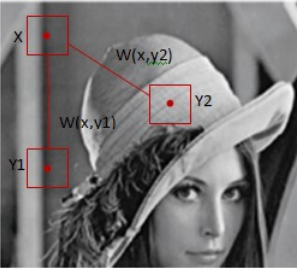
\includegraphics[height=4cm , width=.3\textwidth]{NLmeans.jpg}
     \caption{Principe de l’algorithme NL-Means.}
\end{figure}
\subsection{Algorithme NL-Means}
L’algorithme NLM est un algorithme de débruitage par moyenne
pondérée, dont le noyau qui forme les poids évalué sur la distance entre des voisinages de ces pixels (patchs). Les poids w(x, y) étant normalisés, nous obtenons :
\newline
$$\sum_{y \in \Omega_{x}} w(x, y)=1$$\newline
Dans I'algorithme N-L means, I'image débruitée est estimée selon:
\newline
$$N L M(x)=\sum_{y \in \Omega_{x}} \frac{1}{Z(x)} e^{-\frac{\| P(x)-P(y) \|_{2, a}^{2}}{2 h^{2}}} v(y)$$
\newline
avec
\newline
$Z:$ le facteur de normalisation,
\newline
$P(x):$ le path au pixel $x$ fixé,
\newline $P(y):$ les patchs similaires à $P(x)$,\newline
$h:$ le paramètre de contrôle du degré de lissage.\newline
\section{Conclusion}
Le filtrage représente une opération importante dans le traitement d’images, car il permet
de restaurer l’image originale après une détérioration (bruitage).\newline
Comme plusieurs types de bruits peuvent affecter une image, les traiteurs d’images ont
développé plusieurs types de filtres à cet effet.



\newpage

\chapter{}
\section{Introduction}
Le choix du filtre pour le débruitage d’images numériques reste encore un défi
scientifique pour les chercheurs. Il y a un bon nombre de techniques en traitement d'images
disponibles à appliquer et supprimer le bruit dans une image. Dans notre étude nous nous
intéressons aux quatre types de filtrage (median, min,max et non local means)et un type de bruit (bruit gaussian) .\newline
Nous présentons dans ce chapitre les résultats de comparaison des méthodes de
débruitage sur des images au niveau gris et en couleur a l'aide de PNSR.
\newline
\section{ Rapport crête signal sur bruit (PSNR)}
PSNR (sigle de Peak Signal to Noise Ratio) est une mesure de distorsion utilisée en image numérique, tout particulièrement en compression dimage. Elle permet de quantifier la performance des codeurs en mesurant la qualité de reconstruction de rimage compressée par rapport à rimage originale.

Le $P S N R$ est défini par la formule suivante .
$$
P S N R=10 \cdot \log _{10}\left(\frac{d^{2}}{E Q M}\right)
$$
où $d$ est la dynamique du signal (la valeur maximum possible pour un pixel), dans le cas standard d'une image codée sur 8 bits, $d=255$

EQM est rerreur quadratique moyenne, elle est définie pour 2 images $I_{o}$ et $I_{r}$ de taille $m \times n$ par la formule suivante .
$$
E Q M=\frac{1}{m n} \sum_{i=0}^{m-1} \sum_{j=0}^{n-1}\left(I_{o}(i, j)-I_{r}(i, j)\right)^{2}
$$
\begin{figure}
  \begin{minipage}[t]{0.45\textwidth} %trying to force figs apart
    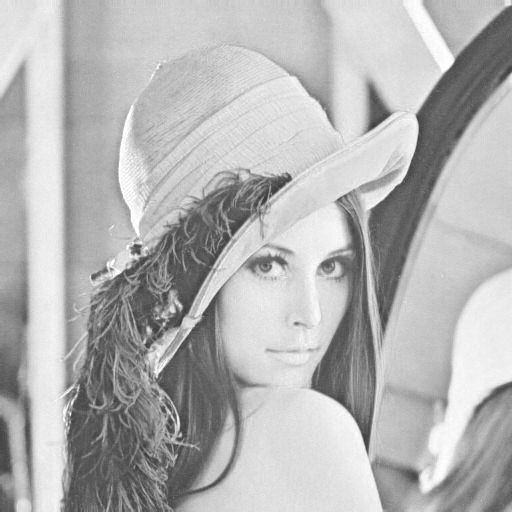
\includegraphics[width=\linewidth]{lena.jpg}
    \caption{Image Originale}
  \end{minipage}%
  \hfill
  \begin{minipage}[t]{0.45\textwidth}
    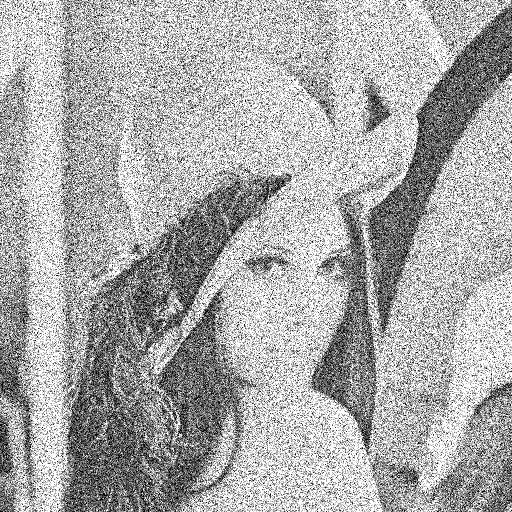
\includegraphics[width=\linewidth]{lena_bruit_gaussien_alpha.jpg}
    \caption{Image avec le bruit gaussien ajouté par xnview sigma=5}
  \end{minipage}
\end{figure}
\begin{figure}
  \begin{minipage}[t]{0.45\textwidth} %trying to force figs apart
    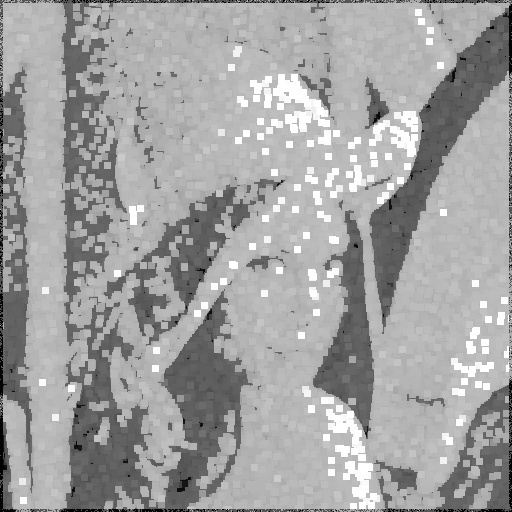
\includegraphics[width=\linewidth]{max_gauss_gris.jpg}
    \caption{Débruitage sur l’image Lena par la méthode max.\newline \newline La valeur PSNR est 28.743817792511383 dB.}
  \end{minipage}%
  \hfill
  \begin{minipage}[t]{0.45\textwidth}
    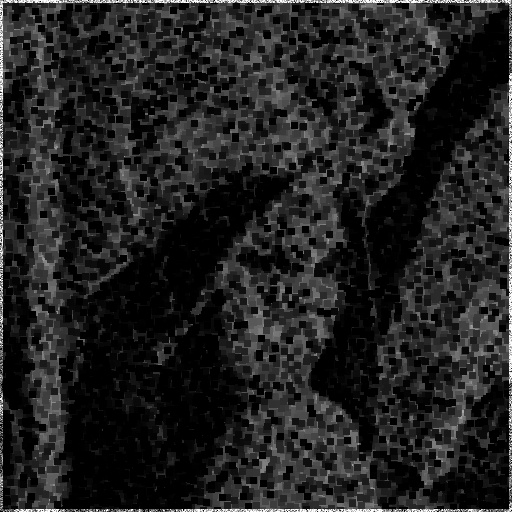
\includegraphics[width=\linewidth]{min_gauss_alpha.jpg}
    \caption{Débruitage sur l’image Lena par la méthode mix.\newline \newline La valeur PSNR est 28.07497953463788 dB.}
  \end{minipage}
\end{figure}
\begin{figure}
  \begin{minipage}[t]{0.45\textwidth} %trying to force figs apart
    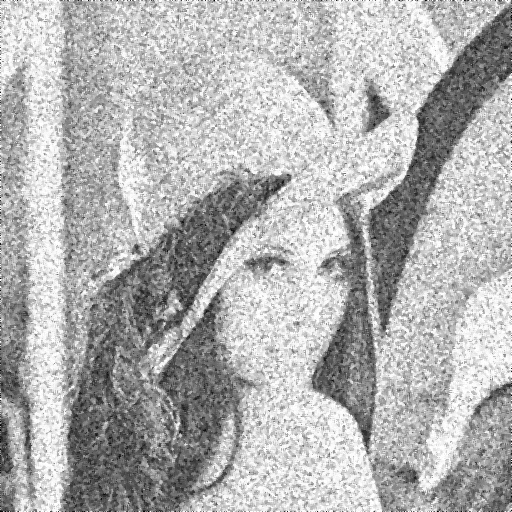
\includegraphics[width=\linewidth]{3x3median_gauss_alpha.jpg}
    \caption{Débruitage sur l’image Lena par la méthode.\newline \newline La valeur PSNR est median 28.560580221588815 dB dB.}
  \end{minipage}%
  \hfill
  \begin{minipage}[t]{0.45\textwidth}
    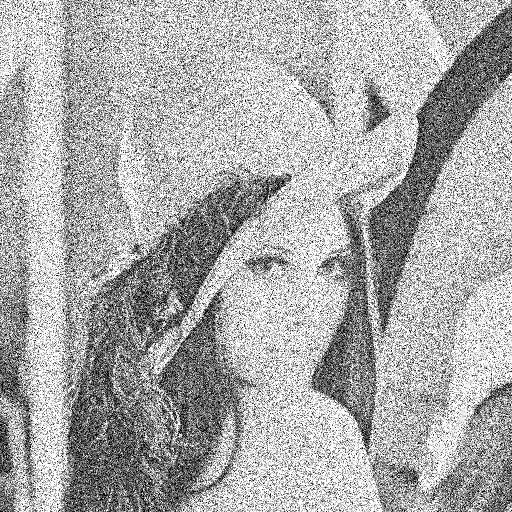
\includegraphics[width=\linewidth]{nlmeans1_gauus_alpha.jpg}
    \caption{Débruitage sur l’image Lena par la méthode nlmeans.\newline \newline La valeur PSNR est 42.792701059859255 dB.}
  \end{minipage}
\end{figure}
\begin{figure}
\newline
\newline
La valeur PSNR 42.792701059859255 dB est le plus couramment utilisé pour estimer l'efficacité des compresseurs, des filtres, etc. Plus la valeur du PSNR est élevée, plus la méthode de compression ou de filtrage correspondante est efficace.
\end{figure}

\newpage
\section{Conclusion}
\newpage
\section{Bibliographie}
\newpage
\section{ANNEXES}

\end{document}







\begin{document}

\maketitle

\section{Introduction}

\end{document}
